\chapter{Решение}
\section{Собственные функции}
Для последующих действий необходимо представить функцию $U$ из задачи \eqref{eq:new_problem} в виде разложения по собственным функциям. Сначала найдем собственные функции. Для этого решим задачу Штурма-Лиувилля.\\
Представим функцию $U$ в форме  
\begin{equation}
  \label{func:form}
  U(y, z, t) = T(t)Y(y)Z(z).
\end{equation}

Рассмотрим однородное уравнение
\begin{equation}
  \label{eq:uniform}
  \frac{1}{c^2} \frac{\partial^2 U}{\partial t^2} = \Delta_{yz} U.\\
\end{equation}

Подставив \eqref{func:form} в \eqref{eq:uniform}, получим
\begin{equation}
  \label{eq:equality}
  \frac{1}{c^2}\frac{T''}{T} = \frac{Y''}{Y} + \frac{Z''}{Z} = -(\lambda^2 + \mu^2).\\
\end{equation}

Здесь $\lambda^2 = \const, \mu = \const$ в силу того, что левая часть \eqref{eq:equality} зависит только от $t$,
а правая~--- от $y$ и $z$. Отсюда следует, что
\begin{equation}
  \label{eq:shturm-liuville}
  \left.
  \begin{array}{rcl}
    Y'' + \lambda^2 Y &=& 0,\\
    Z'' + \mu^2 Z &=& 0,\\
    T'' + c^2(\lambda^2 + \mu^2)T &=& 0.
  \end{array}
  \right.
\end{equation}

Подставив, кроме того, \eqref{func:form} в граничные условия \eqref{eq:new_problem} получим условия
\begin{equation}
  \left.
  \label{eq:conditions}
  \begin{array}{rcl}
    Y(0) &=& 0,\qquad Y(l_y) = 0,\\
    Z(0) &=& 0,\qquad Z(l_y) = 0.
  \end{array}
  \right.
\end{equation}

Таким образом, использовав \eqref{eq:shturm-liuville} и \eqref{eq:conditions}, мы получим две задачи о собственных значениях (задачи Штурма-Лиувилля) для $Y$ и $Z$.
\begin{equation}
  \label{eq:shturm-liuville-final}
  \begin{array}{ll}
    \left\{
      \begin{array}{l}
        Y'' + \lambda^2Y = 0, \\
        Y(0) = Y(l_y) = 0;
      \end{array}
    \right.
    \left\{
      \begin{array}{l}
        Z'' + \mu^2Z = 0, \\
        Z(0) = Z(l_z) = 0.
      \end{array}
    \right.  
  \end{array}
\end{equation}

Решим первую задачу из системы \eqref{eq:shturm-liuville-final}. Как известно (см. \cite{samarsky}) общее решение такого уравнения представимо в виде
\begin{equation}
  \label{eq:common-solution}
  Y(y) = A\sin{\lambda y} + B\cos{\lambda y}.
\end{equation}

Первое граничное условие $Y(0) = 0$ дает нам $B = 0$. Из второго условия $Y(l_y) = 0$ следует 
\[
Y(l_y) = A\sin{\lambda l_y} = 0.
\]

Поскольку $Y(y)$ не равно тождественно нулю, то $A \ne 0$, значит
\begin{equation}
  \label{eq:sin}
  \sin{\lambda l_y} = 0.
\end{equation}

Из \eqref{eq:sin} следует, что $\lambda = \cfrac{\pi n}{l_y}$.

Аналогично решаем вторую задачу системы \eqref{eq:shturm-liuville-final} и получаем нетривиальные решения
\begin{equation}
  \label{func:eigen}
  \begin{array}{ll}
    \left\{
      \begin{array}{l}
        Y = A\sin\lambda y, \\
        \lambda = \frac{\pi n}{l_y},
      \end{array}
    \right.
    \left\{
      \begin{array}{l}
        Z = B\sin\mu z, \\
        \mu = \frac{\pi m}{l_z}.
      \end{array}
    \right.  
  \end{array}
\end{equation}

\section{Получение решения}

Таким образом, $U$ можно представить в виде следующего двойного ряда Фурье по функциям \eqref{func:eigen}.
\begin{equation}
  \label{eq:u-series}
  U(y, z, t) = \displaystyle \sum_{m=1}^{\infty}\sum_{n=1}^{\infty} \gamma(t) \sin\frac{\pi n y}{l_y} \sin\frac{\pi m z}{l_z}.
\end{equation}
\\
Разложим собственным функциям \eqref{func:eigen} неоднородную правую часть $G(y, z, t)$ системы \eqref{eq:new_problem} и функцию $\Phi(y, z)$. В дальнейших рассуждениях для простоты умножим левую и правую части первого уравнения \eqref{eq:new_problem} на $c^2$, получив
\begin{equation}
  \label{eq:new_eq_simple}
  \frac{\partial^2 U}{\partial t^2} = \Delta_{yz} U + c^2G(y, z, t)
\end{equation}

\begin{enumerate}
\item Разложение $G(y, z, t)$.
  Разложим функцию $G(y, z, t) = \pi^2 c^2\frac{l_z - z}{lz}\frac{4l_y^2 - \lambda^2}{\lambda^2 \l_y^2}\sin\frac{2\pi c}{\lambda}t \sin\frac{\pi y}{l_y}$ по функциям \eqref{func:eigen}. Заметим, что функция $G$ уже содержит в себе собственную функцию $\sin\frac{\pi y}{l_y}$, значит, необходимо разложить лишь зависящую от $z$ часть. Разложение будет иметь вид
  \begin{equation}
    \label{func:G_represent}
    G(y, z, t) =  \pi^2 c^2 \frac{4l_y^2 - \lambda^2}{\lambda^2 \l_y^2} \sin\frac{2\pi c}{\lambda}t\displaystyle \sum_{m=1}^{\infty}  g_{nm}^{(z)}(t) \sin\frac{\pi y}{l_y} \sin\frac{\pi m z}{l_z}.
  \end{equation}
  Найдем коэффициенты ряда.
%   \begin{equation}
%     \label{func:g}
%     \begin{array}{rcl}
%       g^{(z)}_{nm}(t) &=& \frac{2}{l_z} \displaystyle \int_0^{l_z} \frac{l_z - z}{l_z} \sin\frac{\pi m z}{l_z} dz
%       =\frac{2}{l_z}\left[\int_0^{l_z}\sin\frac{\pi m z}{l_z}dz - \int_0^{l_z}\frac{z}{l_z} \sin\frac{\pi m z}{l_z}dz\right] =\\
%       \\
%       &=& \frac{2}{l_z} \left[ \left. -\frac{l_z}{\pi m} \cos\frac{\pi m z}{l_z}\right|_{0}^{l_z} - \left. \frac{z l_z}{\pi m}\cos\frac{\pi m z}{l_z}\right|_{0}^{l_z} + \int_0^{l_z}\frac{l_z}{\pi m}\cos\frac{\pi m z}{l_z}dz\right] =\\
%       \\
%       &=& \frac{2}{l_z}\frac{l_z}{\pi m} \left( 1 - (-1)^m - (-1)^{m+1} \right) = \frac{2}{\pi m}.
%     \end{array}
%   \end{equation}
  \begin{eqnarray}
    \nonumber
    g^{(z)}_{nm}(t) &=& \frac{2}{l_z} \displaystyle \int_0^{l_z} \frac{l_z - z}{l_z} \sin\frac{\pi m z}{l_z} dz = \frac{2}{l_z}\left[\int_0^{l_z}\sin\frac{\pi m z}{l_z}dz - \int_0^{l_z}\frac{z}{l_z} \sin\frac{\pi m z}{l_z}dz\right] =\\
    \nonumber
    &=& \frac{2}{l_z} \left[ \left. -\frac{l_z}{\pi m} \cos\frac{\pi m z}{l_z}\right|_{0}^{l_z} - \left. \frac{z l_z}{\pi m}\cos\frac{\pi m z}{l_z}\right|_{0}^{l_z} + \int_0^{l_z}\frac{l_z}{\pi m}\cos\frac{\pi m z}{l_z}dz\right] =\\
    \label{func:g}
    &=& \frac{2}{l_z}\frac{l_z}{\pi m} \left( 1 - (-1)^m - (-1)^{m+1} \right) = \frac{2}{\pi m}.
  \end{eqnarray}
  
  Подставив разложение \eqref{func:g} в \eqref{func:G_represent} получим
  \begin{equation}
    \label{func:G}
    G(y, z, t) = 2\pi c^2\frac{4l_y^2 - \lambda^2}{\lambda^2 \l_y^2} \sin\frac{2\pi c}{\lambda}t\displaystyle \sum_{m=1}^{\infty}\frac{1}{m}\sin\frac{\pi y}{l_y} \sin\frac{\pi m z}{l_z}.
  \end{equation}

\item Разложение начального условия.


  Для удобства введем замену $k = \frac{2\pi c}{\lambda}$. Теперь разложим начальное условие  $\Phi(y, z, t) = -k\frac{l_z - z}{l_z}\sin\frac{\pi y}{l_y}$. Как и в предыдущем случае, она уже разложена по собственным функциям относительно $y$, будем искать разложение относительно $sin\frac{\pi m z}{l_z}$. Разложения будет иметь следующий вид
  \[
  \Phi(y, z, t) = \displaystyle -k\sum_{m=1}^{\infty}\varphi(t) \sin\frac{\pi y}{l_y} \sin\frac{\pi m z}{l_z}.
  \]
  Найдем коэффициенты разложения
  \begin{eqnarray*}
    \varphi(t) = \displaystyle \frac{2}{l_z} \int_0^{l_z} \frac{l_z - z}{l_z}\sin\frac{\pi m z}{l_z}dz = \frac{2}{\pi m}.
  \end{eqnarray*}
  Таким образом
  \[
  \Phi(y, z, t) = -\frac{2k}{\pi}\displaystyle \sum_{m=1}^{\infty} \frac{1}{m} \sin\frac{\pi y}{l_y} \sin\frac{\pi m z}{l_z}.
  \]
\end{enumerate}

Подставим все полученные разложения и учтем, что правая часть и начальное условие не являются нулевыми лишь при $n = 1$, поэтому и разложение $U(y, z, t)$ представим в виде обыкновенного ряда Фурье.
\[
U(y, z, t) = \displaystyle \sum_{m=1}^{\infty} \gamma(t) \sin\frac{\pi y}{l_y} \sin\frac{\pi m z}{l_z}.
\]
Подставив в систему разложения и приравняв коэффициенты при одинаковых базисных функциях, получим систему обыкновенных дифференциальных уравнений с начальными условиями вида
\[
\left\{
    \begin{array}{l}
      \gamma''(t) + w^2_{m}\gamma(t) = \frac{2\pi c^2}{m}\left(\frac{4l_y^2 - \lambda^2}{l_y^2\lambda^2} \right)\sin{kt},\\
      \begin{array}{rcl}
      \gamma(0) &=& 0,\\
      \gamma'(0) &=& -\frac{2k}{\pi m}.
      \end{array}
    \end{array}
\right.
\]\\
Здесь $w_{m} = \pi c \sqrt{\frac{1}{l_y^2} + \frac{m^2}{l_z^2}}$\\
Найдем общее решение соответствующего однородного уравнения
\[
\begin{array}{l}
  \gamma''(t) + w^2_{m}\gamma(t) = 0,\\
  \gamma^{0}(t) = A\cos{w_m t} + B\sin{w_mt}.
\end{array}
\]
Рассмотрим теперь неоднородную задачу и найдем ее частное решение. Исходя из вида правой части, вид решения будет таким
\[
\tilde{\gamma}(t) = C\cos{kt} + D\sin{kt}.
\]
Подставим функцию такого вида в уравнение и получим
\[
-k^2C\cos{kt} - k^2 D\sin{kt} + w^2_m C\cos{kt} + w^2_{m} D\cos{kt} = \frac{2\pi c^2}{m}\left(\frac{4l_y^2 - \lambda^2}{l_y^2\lambda^2} \right)\sin{kt}.
\]
Приравняем коэффициенты при соответствующих функциях и получим систему
$\begin{equationsset}
      (w_m^2 - k^2)C & = & 0, \\
      (w_m^2 - k^2)D & = & \frac{2\pi c^2}{m}\left(\frac{4l_y^2 - \lambda^2}{l_y^2\lambda^2} \right).
\end{equationsset}$
      

Отсюда $C = 0$, $D = \frac{2\pi c^2}{m(w_m^2 - k^2)}\left(\frac{4l_y^2 - \lambda^2}{l_y^2\lambda^2} \right)$.\\
Общее решение выглядит как сумма общего решения однородного уравнения и частного решения неоднородного, то есть
\[
\gamma(t) = A\cos{w_mt} + B\sin{w_mt} + \frac{2\pi c^2}{m(w_m^2 - k^2)}\left(\frac{4l_y^2 - \lambda^2}{l_y^2\lambda^2} \right)\sin{kt}.
\]
Используем начальные условия и получим систему
\[
\left\{
  \begin{array}{l}
    A = 0,\\
    w_nB + kD = -\frac{2k}{\pi m} \Rightarrow B = -\frac{k}{w_m}\left(\frac{2}{\pi m} + D \right).
  \end{array}
\right.
\]
Таким образом,
\begin{eqnarray*}
  \gamma(t) &=& \frac{2\pi c^2}{m(w_m^2 - k^2)}\left(\frac{4l_y^2 - \lambda^2}{l_y^2\lambda^2} \right)\sin{kt} - \frac{k}{w_m}\left(\frac{2}{\pi m} + D\right)\sin{w_mt},\\
  U(y, z, t) &=& \displaystyle \sum_{m=1}^{\infty} \left( \frac{2\pi c^2}{m(w_m^2 - k^2)}\left(\frac{4l_y^2 - \lambda^2}{l_y^2\lambda^2} \right)\sin{kt} - \frac{k}{w_m}\left(\frac{2}{\pi m} + D\right)\sin{w_mt} \right) \sin\frac{\pi y}{l_y} \sin\frac{\pi m z}{l_z},\\
  E_x(y, z, t) &=& \displaystyle
    \sum_{m=1}^{\infty} \left( \frac{2\pi c^2}{m(w_m^2 - k^2)}\left(\frac{4l_y^2 - \lambda^2}{l_y^2\lambda^2} \right)\sin{kt} - \frac{k}{w_m}\left(\frac{2}{\pi m} + D\right)\sin{w_mt} \right) \sin\frac{\pi y}{l_y} \sin\frac{\pi m z}{l_z}\\
    &+& \frac{l_z - z}{l_z} \sin\frac{2\pi c}{\lambda}t \sin\frac{\pi y}{l_y}
\end{eqnarray*}

\begin{figure}[!hbtp]
  \center
  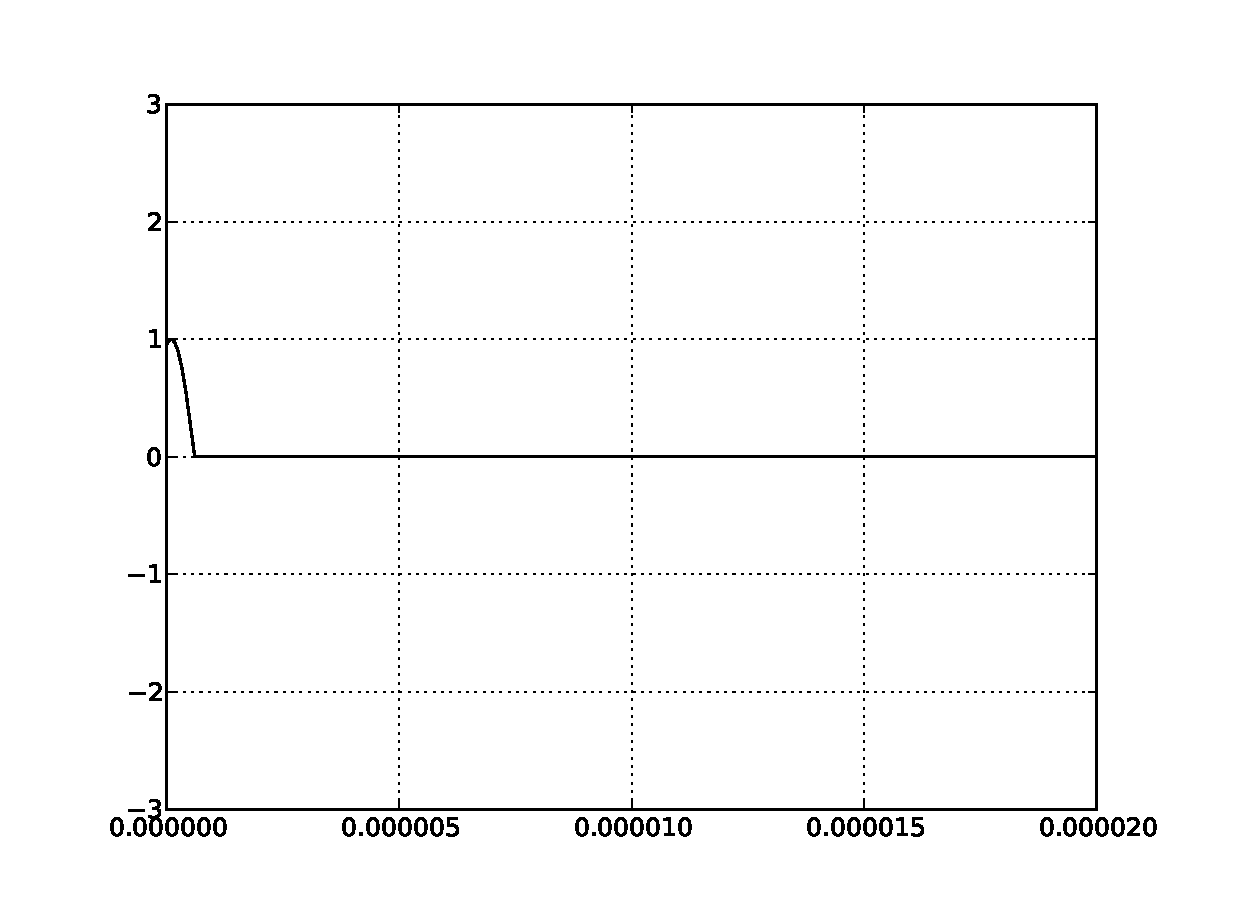
\includegraphics[width=0.9\linewidth]{first}
  \caption{Волна в момент $t = 2\cdot10^{-15}$}
\end{figure}

\begin{figure}[!hbtp]
  \center
  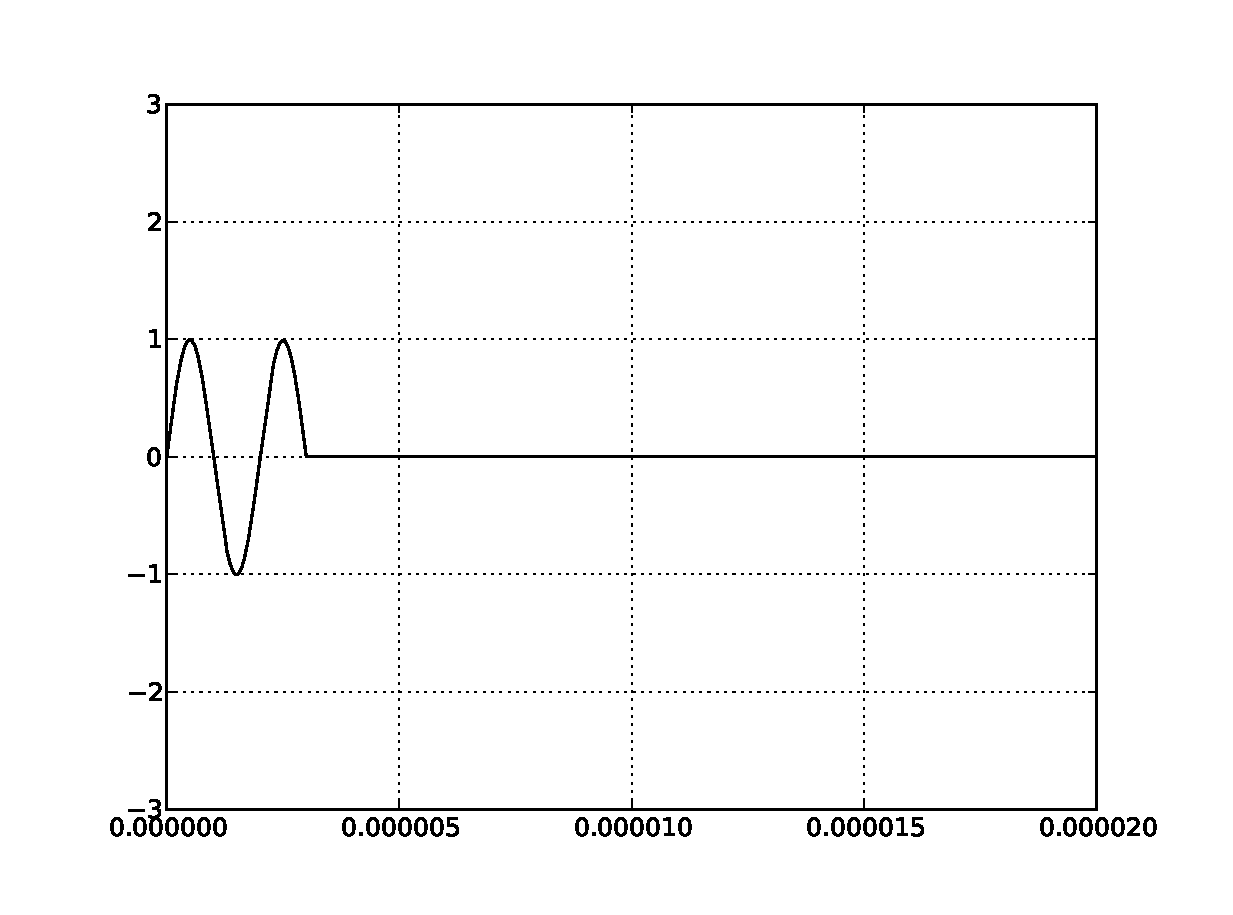
\includegraphics[width=0.9\linewidth]{second}
  \caption{Волна в момент $t = 1\cdot10^{-14}$}
\end{figure}

\begin{figure}[!hbtp]
  \center
  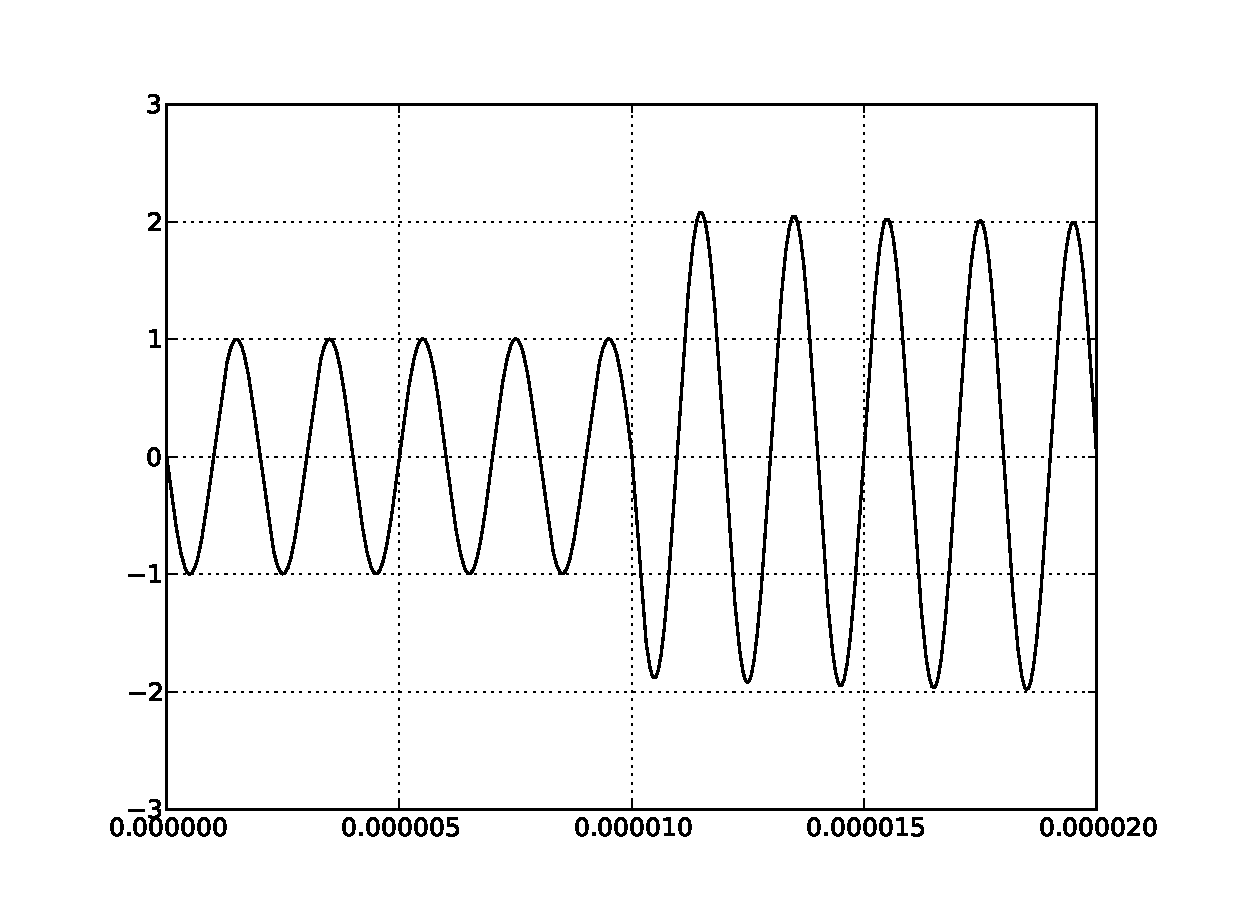
\includegraphics[width=0.9\linewidth]{third}
  \caption{Волна в момент $t = 1\cdot10^{-13}$}
\end{figure}
